

\section{Method}
\begin{figure}
   \centering
   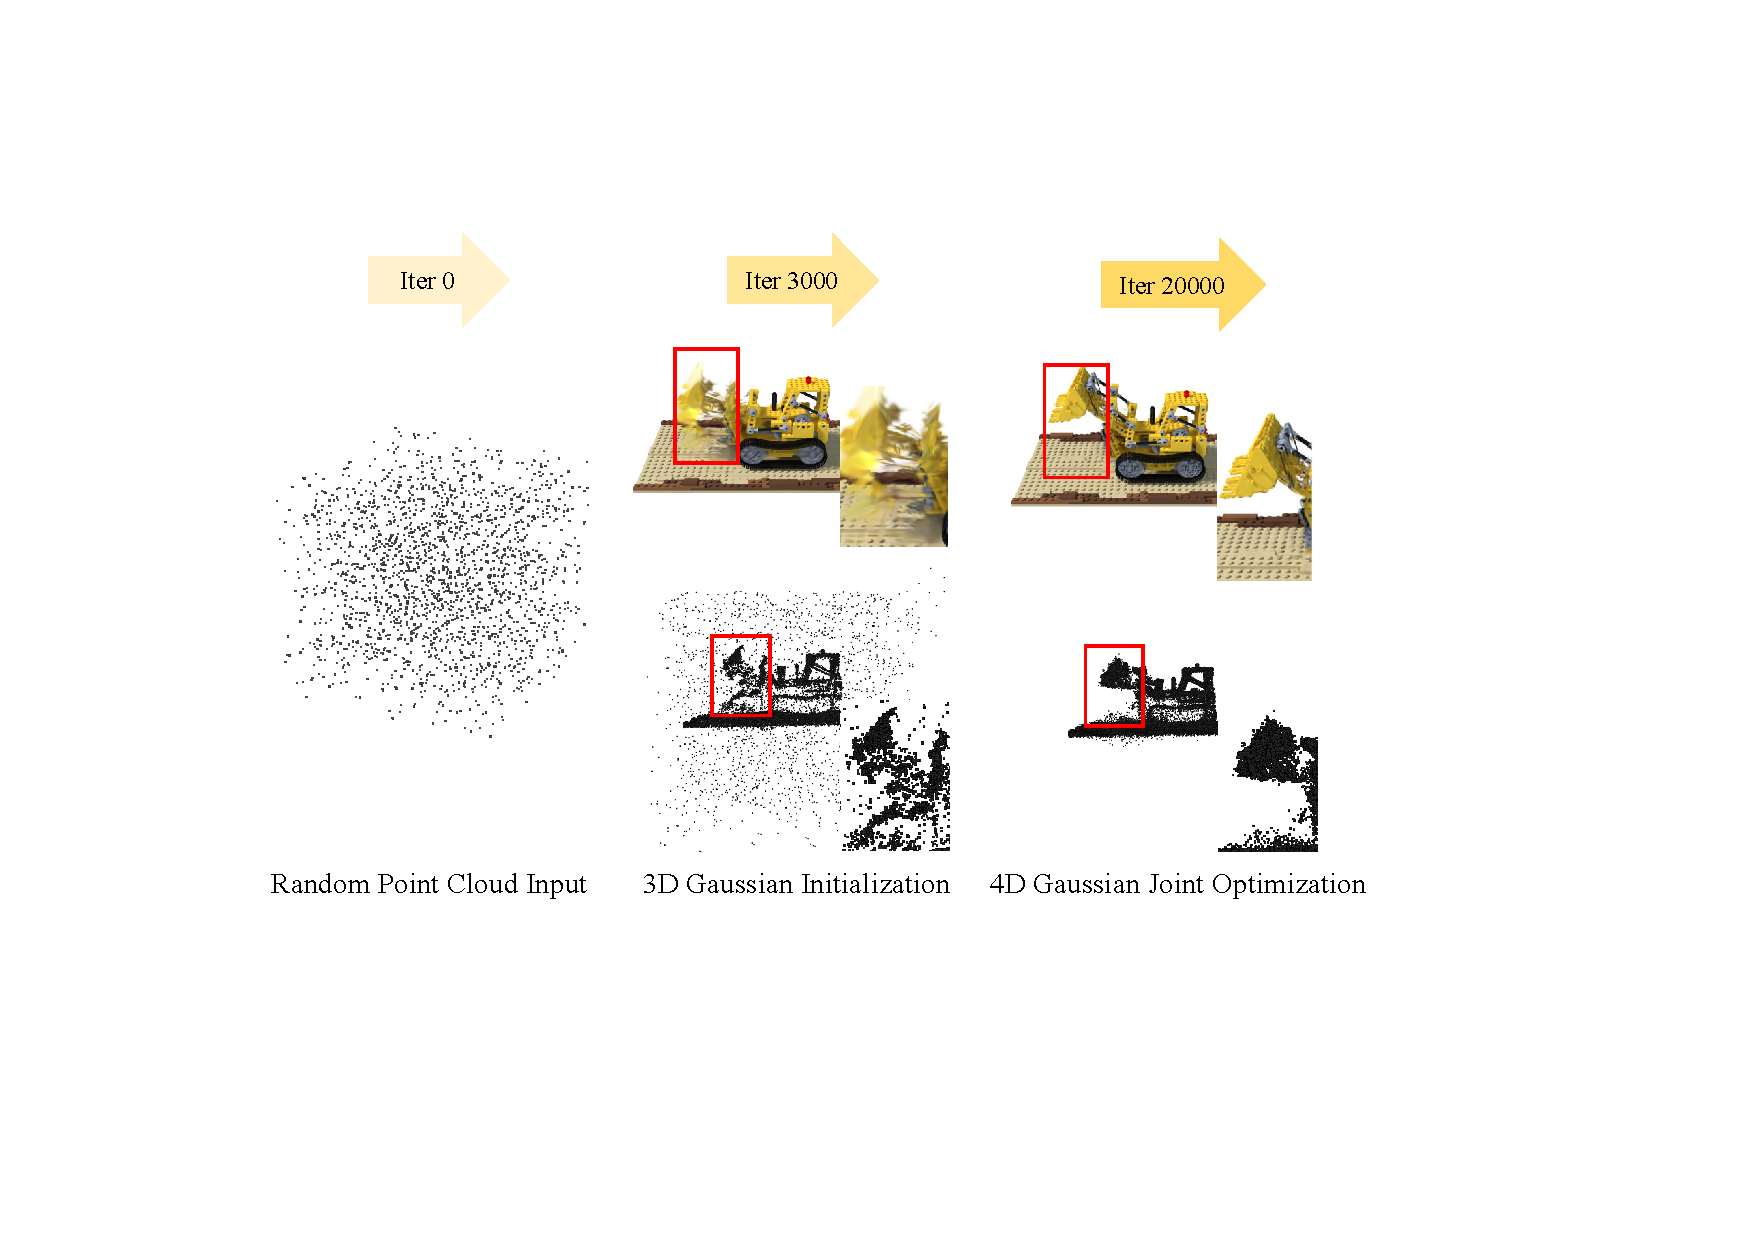
\includegraphics[width=\linewidth]{fig/coarse2fine.pdf}
   \caption{Illustration of the optimization process. With static 3D Gaussian initialization, our model can learn high-quality 3D Gaussians of the motion part. }
   \label{fig: coarse2fine}
   \vspace{-10pt}
\end{figure}
% framework
    % -->>>>>编码时间的变化,
    % -->>>>>canonical space mapping
    % -->>>>>encode both position and shape deformation
% deformation fields
    % to capture both nearby and far-distance movement, multi-resolution voxel planes are considered.
    % The motion of each point is very direct, so a tiny MLP is strong enough to decode the information.
% optimization
    % two-stage training
    % TV Loss
Sec.~\ref{subsec:4dgs} introduces the overall 4D Gaussian Splatting framework. Then, the Gaussian deformation field is proposed in Sec.~\ref{subsec:filed}. Finally, we describe the optimization process in Sec.~\ref{subsec:optimization}. 

\subsection{4D Gaussian Splatting Framework}
\label{subsec:4dgs}
% Adopting a deformation field to encode 4D information is a common approach in related works~\cite{pumarola2021dnerf,tineuvox}. Given a rendered pixel, a ray $r$ is cast. The sampled points $x$ and timestamp $t$ are fed into an MLP to map into a canonical space and applied with volume rendering~\cite{drebin1988volume}. However, each point on the sample ray may own different velocity variables, which causes heavily different deformation, as shown in Fig.~\ref{fig: splatting-volume}, after applying canonical mapping, the position of each ray is changed. so the volume rendering process may become inaccurate. Meanwhile, differential splatting~\cite{yifan2019differentiablesplatting} creates a relationship among 3D Gaussians on the rendered pixel directly, therefore, each rendered pixel may influenced by different 3D Gaussians every timestamp. The differential splatting is still meaningful. Therefore, we only maintain one set of canonical 3D Gaussians, what we need to do is to employ deformation fields $\mathcal{F}$ to predict each 3D Gaussian's state at a given timestamp $t$.

As shown in Fig.~\ref{fig: pipeline}, given a view matrix $M=[R, T]$, timestamp $t$, our 4D Gaussian splatting framework includes 3D Gaussians $\mathcal{G}$ and Gaussian deformation field network $\mathcal{F}$. Then a novel-view image $\hat{I}$ is rendered by differential splatting~\cite{yifan2019differentiablesplatting} $\mathcal{S}$ following $\hat{I} = \mathcal{S}(M,\mathcal{G}^\prime)$, where $\mathcal{G}^\prime=\Delta\mathcal{G}+\mathcal{G}$.

Specifically, the deformation of 3D Gaussians $\Delta \mathcal{G}$ is introduced by the Gaussian deformation field network $\Delta \mathcal{G} = \mathcal{F}(\mathcal{G}, t)$, in which the spatial-temporal structure encoder $\mathcal{H}$ can encode both the temporal and spatial features of 3D Gaussians $f_d=\mathcal{H}(\mathcal{G}, t)$, and the multi-head Gaussian deformation decoder $\mathcal{D}$ can decode the features and predict each 3D Gaussian's deformation $\Delta \mathcal{G} = \mathcal{D}(f)$, then the deformed 3D Gaussians $\mathcal{G}^\prime$ can be introduced.

% Finally, differential Gaussian splatting~\cite{yifan2019differentiablesplatting} is applied to the deformed 3D Gaussians to render a novel view image.

The rendering process of our 4D Gaussian Splatting is depicted in Fig.~\ref{fig: splatting-volume}~\textcolor{red}{(c)}. Our 4D Gaussian splatting converts the original 3D Gaussians $\mathcal{G}$ into another group of 3D Gaussians $\mathcal{G}^\prime$ given a timestamp $t$, maintaining the effectiveness of the differential splatting as referred in~\cite{yifan2019differentiablesplatting}.

% \begin{figure}
%    \centering
%    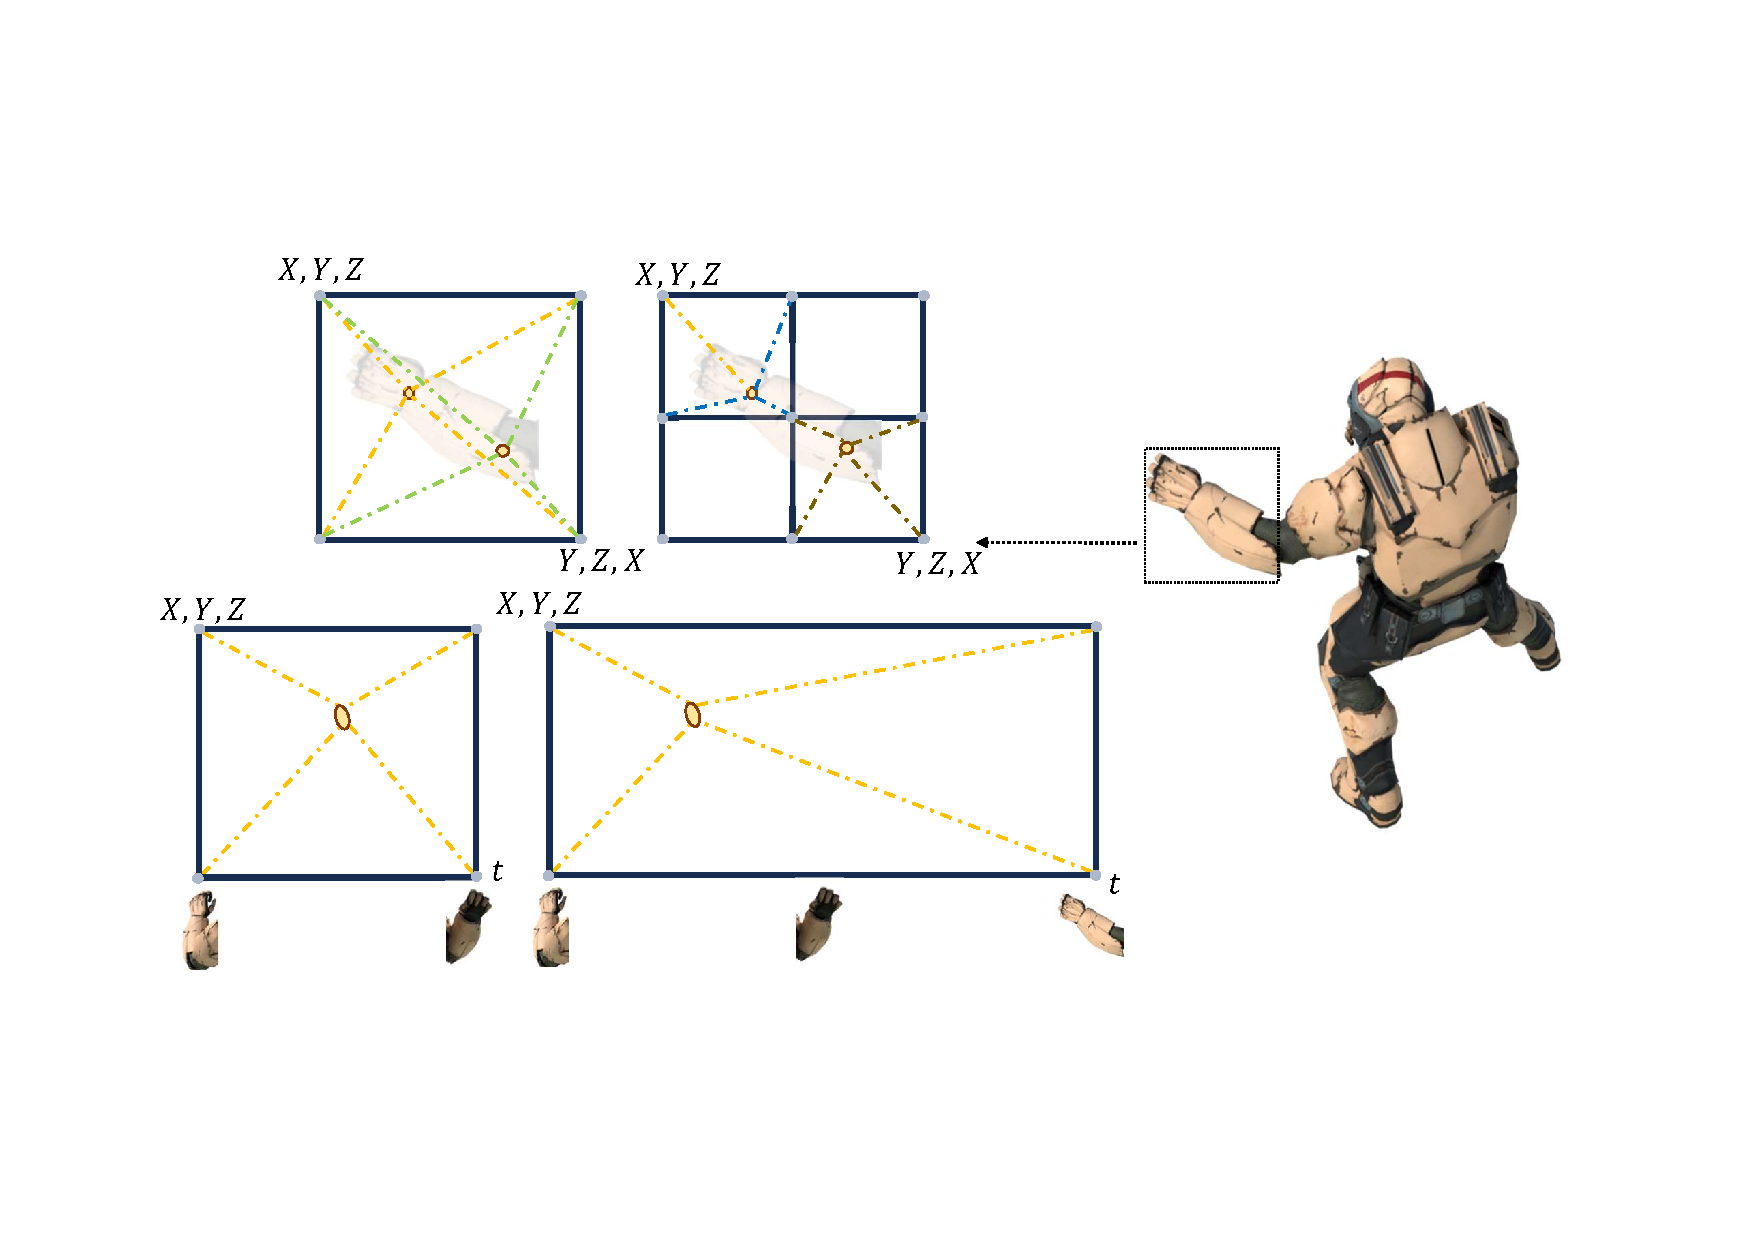
\includegraphics[width=1.0\linewidth]{fig/voxelgrid.pdf}
%    \caption{Illustration of querying multi-resolution voxel grids.}
%    \label{fig: voxelgrid}
% \end{figure}




\begin{figure*}
   \centering
   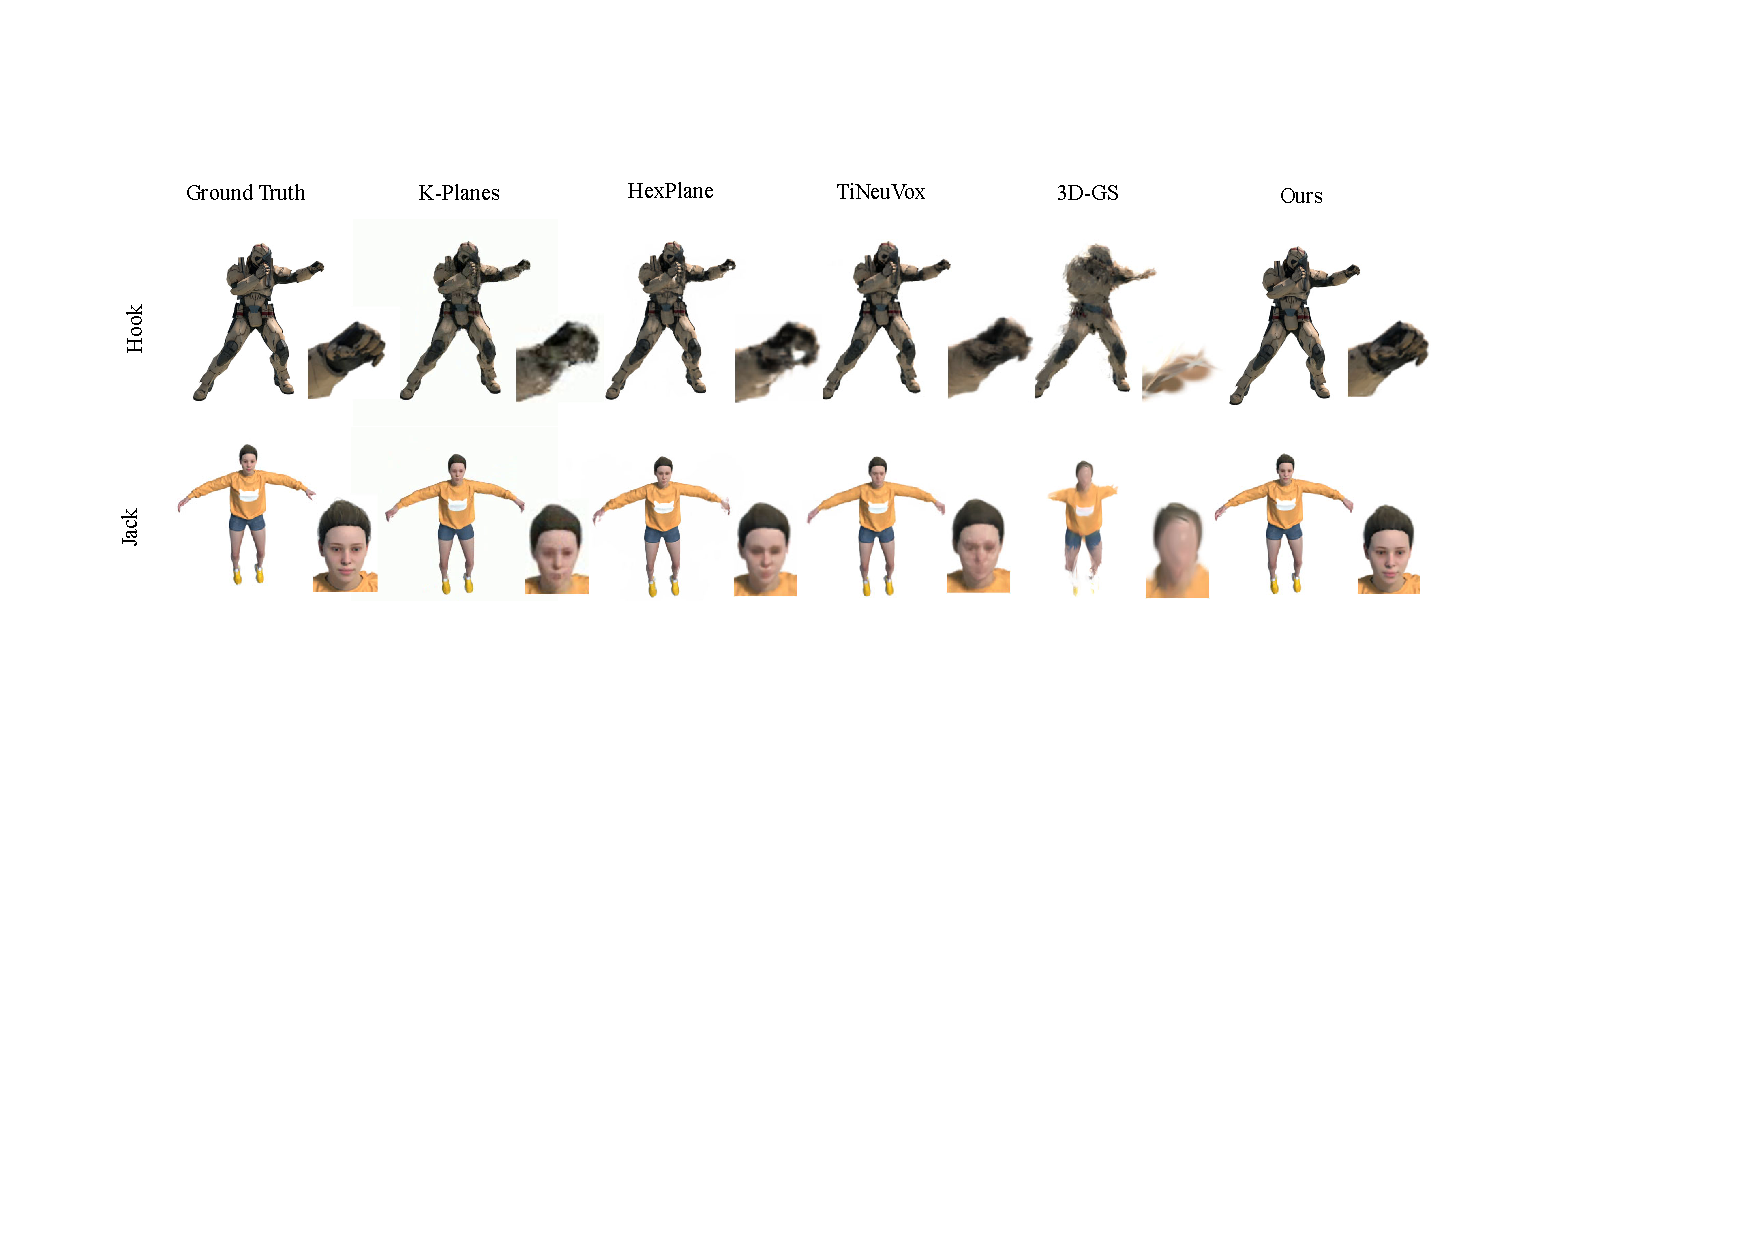
\includegraphics[width=1.0\linewidth]{fig/dnerf_result.pdf}
   \caption{Visualization of synthesized datasets compared with other models~\cite{hexplane,kplanes,tineuvox,3dgs,guo2023forwardflowfornvs,msth}. The rendering results of~\cite{kplanes} are displayed with a default green background. We have adopted their rendering settings.}
      \label{fig: dnerf_result}
      \vspace{-10pt}
\end{figure*}

\subsection{Gaussian Deformation Field Network}
\label{subsec:filed}

The network to learn the Gaussian deformation field includes an efficient spatial-temporal structure encoder $\mathcal{H}$ and a Gaussian deformation decoder $\mathcal{D}$ for predicting the deformation of each 3D Gaussian.

\paragraph{Spatial-Temporal Structure Encoder.}

Nearby 3D Gaussians always share similar spatial and temporal information. To model 3D Gaussians' features effectively, we introduce an efficient spatial-temporal structure encoder $\mathcal{H}$ including a multi-resolution HexPlane $R(i,j)$ and a tiny MLP $\phi_d$ inspired by ~\cite{tineuvox,hexplane,kplanes,tensor4d}. While the vanilla 4D neural voxel is memory-consuming, we adopt a 4D K-Planes~\cite{kplanes} module to decompose the 4D neural voxel into 6 planes. All 3D Gaussians in a certain area can be contained in the bounding plane voxels and Gaussian's deformation can also be encoded in nearby temporal voxels.
% To compute the features of 3D Gaussians, bilinear interpolation is employed, which also models the relationship of nearby 3D Gaussians. 

Specifically, the spatial-temporal structure encoder $\mathcal{H}$ contains 6 multi-resolution plane modules $R_l(i,j)$ and a tiny MLP $\phi_d$, \ie $\mathcal{H}(\mathcal{G},t)=\{R_l(i,j), \phi_d | (i,j) \in \{(x,y),(x,z),(y,z),(x,t),(y,t),(z,t)\}, l \in \{1,2\}\}$. The position $\mathcal{X} = (x,y,z)$ is the mean value of 3D Gaussians $\mathcal{G}$. Each voxel module is defined by $R(i,j)\in \mathbb{R}^{h\times l N_i \times l N_j}$, where $h$ stands for the hidden dim of features, $N$ denotes the basic resolution of voxel grid and $l$ equals to the upsampling scale. 
This entails encoding information of the 3D Gaussians within the 6 2D voxel planes while considering temporal information. The formula for computing separate voxel features is as follows:
\begin{equation}
\begin{aligned}
  % f_{voxel} &= \mathcal{F}(\mathcal{X},t)\\
  f_h &= \bigcup_l \prod \text{interp}(R_l(i,j)), \\
    (i,j) &\in \{(x,y),(x,z),(y,z),(x,t),(y,t),(z,t)\}. 
\end{aligned}
\label{formula:feature_position}
\end{equation}
$f_{h} \in \mathbb{R}^{h*l}$ is the feature of neural voxels. `interp' denotes the bilinear interpolation for querying the voxel features located at 4 vertices of the grid. The discussion of the production process is similar to~\cite{kplanes}. Then a tiny MLP $\phi_d$ merges all the features by $f_d = \phi_d(f_h)$.

% In the compact representation of 3D Gaussians, the position $\mathcal{X}$ and time $t$ of these 3D Gaussians play a crucial role in encoding their motion. Besides, as shown in Fig.~\ref{fig: coarse2fine}, during the optimization, the point of Gaussians becomes denser, which means that the covariance of 3D Gaussians is decreasing. Meanwhile, when we introduce additional parameters like covariance values $s$ and $r$ into these 3D Gaussians, it increases the computational demands, leading to a slowdown in both rendering and training speeds. So we conclude that the covariance of Gaussians will become less important during the optimization. Therefore, we omit the 3D Gaussian's rotation and scaling information and focus solely on the position $\mathcal{X}$ and given timestamp $t$. 

\paragraph{Multi-head Gaussian Deformation Decoder.}
\label{subsec:Gaussian Deformation Decoder}

When all the features of 3D Gaussians are encoded, we can compute any desired variable with a multi-head Gaussian deformation decoder $\mathcal{D}=\{\phi_x, \phi_r, \phi_s\}$. Separate MLPs are employed to compute the deformation of position $\Delta \mathcal{X} = \phi_x(f_d)$, rotation $\Delta r= \phi_r(f_d)$, and scaling $\Delta s=\phi_s(f_d)$.
Then, the deformed feature $(\mathcal{X}^\prime,r^\prime,s^\prime)$ can be addressed as:
\begin{align}
    & (\mathcal{X}^\prime, r^\prime, s^\prime) = (\mathcal{X} + \Delta \mathcal{X}, r + \Delta r, s + \Delta s) .
\end{align}
Finally, we obtain the deformed 3D Gaussians $\mathcal{G}^\prime=\{\mathcal{X}^\prime, s^\prime, r^\prime,\sigma,\mathcal{C} \}$.


% \paragraph{Empty Voxel Mask Grid for Multi-cams Setups.}
% In the multi-video setups, dynamic scenes can be modelled by 4D-GS precisely and both the motion part and static part can be divided. Therefore, we proposed a empoty voxel mask $\mathcal{M}$ to split the static 3D Gaussians and dynamic 3D Gaussians explicitly. Speficially, all the deformation value $( \Delta \mathcal{X},\Delta r,\Delta s ) $ computed by Gaussian Deformation Decoder will be multipied by a motion ratio tri-linearly interpolated by the explicit voxel grid $\delta = \mathcal{M}(\mathcal{X})$. The deformation of all the 3D Gaussians will be replaced by:
% \begin{align}
%     & (\mathcal{X}^\prime, r^\prime, s^\prime) = (\mathcal{X} + \Delta \mathcal{X}*\delta, r + \Delta r * \delta, s + \Delta s * \delta) .
% \end{align}
% As is shown in Fig.~\ref{fig: empty_voxel_vis}, multi-cams setups can boost 4D-GS decompose static and dynamic part easily, explicit empoty voxel also guided the optimization of model, which contribute to rendering qualities.

% \begin{figure}
%    \centering
%    \includegraphics[width=1.0\linewidth]{fig/voxel_vis.pdf}
%    \caption{Visualization of dynamic scene point clouds and Empty Voxel Mask grid. The colored point stand for non-zero value of the empty voxel mask grid. Note that edged of the scenes only captured by few cameras, which causes failure of modeling.}
%    \label{fig: empty_voxel_vis}
% \end{figure}

    
\subsection{Optimization}
\label{subsec:optimization}



\paragraph{3D Gaussian Initialization.}
\cite{3dgs} shows that 3D Gaussians can be well-trained with structure from motion (SfM)~\cite{schonberger2016structure} points initialization. Similarly, 4D Gaussians should also be fine-tuned in proper 3D Gaussian initialization. We optimize 3D Gaussians at initial 3000 iterations for warm-up and then render images with 3D Gaussians $\hat{I} = \mathcal{S}(M,\mathcal{G})$ instead of 4D Gaussians $\hat{I}=\mathcal{S}(M,\mathcal{G}^\prime)$. The illustration of the optimization process is shown in Fig.~\ref{fig: coarse2fine}.


% Direct optimizing 4D-GS may cause disturbing even failure in both learning the deformation field and 3D Gaussians. So we have to initialize random 3D Gaussians $\mathcal{S}$ in the manually defined bounding box and train the $\mathcal{S}$ only, then 4D Gaussians $\mathcal{G}=\{ \mathcal{S},\mathcal{D},\mathcal{F} \}$ feed activated in the joint optimization process. 



% \begin{algorithm}
%      \caption{Active 3D Gaussians Growing}
%      \label{algorithm: Active 3D Gaussians Growing}
%     \begin{algorithmic}[1]
%      \Require $\mathcal{S}$
%      \Require $N_{down},N_{thres}$
%      \Require $mindis,radii$
%      \Ensure New 3D Gaussians $\mathcal{S}+\mathcal{\hat{S}}$
%      \State  $\mathcal{S}_0 \leftarrow \mathcal{S}$
%      \State  $\mathcal{\hat{S}} \leftarrow \{\}$

%      \While{num of $\mathcal{S}_0 < N_{down}$ }
%         \State $\mathcal{S}_0 \leftarrow $ Downsample($\mathcal{S}_0$)
%      \EndWhile
%      \While{$\hat{S} < N_{thres} $}
%           \ForAll {3D Gaussians $s_i$ in $\mathcal{S}_0$}
%         \State $d$ = SearchNearest($s_i$)
%         \If{ $d>$ $mindis$}
%               \State $\mathcal{\hat{S}} \leftarrow \{\mathcal{\hat{S}}, s_i + radii*random(size=3)\}$ 
%         \EndIf
%         \State $mindis \leftarrow mindis / 2$ 
%         \State $radii \leftarrow radii / 2$ 

        
%      \EndFor
%      \EndWhile

     
%     \end{algorithmic}
% \end{algorithm}


% \paragraph{Active 3D Gaussians Growing.}
% For the unbounded scenes in the feed-forward settings, sfm~\cite{schonberger2016structurefrommotion} cannot reconstruct all the details of the far-distant area. Which cause to fail of optimizing 3DGS and 4DGS. The reason is that splitting \& cloning 3D Gaussians following gradient flow only cannot cover the area which is far from capturing cameras and own less 3D Gaussians provided by sfm. Meanwhile, far-distant 3D Gaussians are always ignored by differential splatting, which lead to the low gradient value and the difficult of 3D Gaussians' growth. 

% To solve the problem, we propose a active 3D Gaussians growing methods to enable 3D Gaussians' growth.
\paragraph{Loss Function.}
Similar to other reconstruction methods~\cite{3dgs,pumarola2021dnerf,tineuvox}, we use the L1 color loss to supervise the training process. A grid-based total-variational loss~\cite{dvgo,tineuvox,hexplane,kplanes} $\mathcal{L}_{tv}$ is also applied.
\begin{equation}
    % \mathcal{L} = \lambda_1(\hat{c} - c)^2 + \lambda_2\mathcal{L}_{ssim}{(\hat{c},c)} + \lambda_3\mathcal{L}_{lpips}{(\hat{c},c)} + \lambda_4  \mathcal{L}_{constraint}.
    \mathcal{L} = \hat{I} - I + \mathcal{L}_{tv}.
\end{equation}
% $\lambda_i$ are hyperparameters can be manually selected before the beginning of training.